\documentclass[11pt,a4paper]{article}
\usepackage[top=2.2cm,bottom=2.2cm,left=2.3cm,right=2.3cm]{geometry}
\usepackage[T1]{fontenc}
\usepackage{newtxtext,newtxmath}
\usepackage{microtype,amsmath,booktabs,array,tabularx,graphicx,xcolor,float,caption,enumitem,longtable,listings,tikz,cite,url}
\usepackage[colorlinks=true,linkcolor=blue!50!black,citecolor=blue!50!black,urlcolor=blue!50!black]{hyperref}
\usepackage{titlesec,fancyhdr}
\usetikzlibrary{arrows.meta,positioning,shapes.geometric,fit,backgrounds}
\definecolor{navy}{HTML}{0B3D6B}
\titleformat{\section}{\Large\bfseries\color{navy}}{\thesection}{0.6em}{}
\titleformat{\subsection}{\large\bfseries\color{navy}}{\thesubsection}{0.6em}{}
\titleformat{\subsubsection}{\normalsize\bfseries}{\thesubsubsection}{0.6em}{}
\setlength{\parindent}{0pt}\setlength{\parskip}{5pt}
\newcolumntype{Y}{>{\raggedright\arraybackslash}X}
\pagestyle{fancy}\fancyhf{}\cfoot{\footnotesize LeakLens: Water Leak Localization System \,|\, \thepage}\renewcommand{\headrulewidth}{0pt}
\captionsetup{font=small,labelfont=bf}
\lstset{basicstyle=\ttfamily\footnotesize,breaklines=true,frame=single,framerule=0.3pt,rulecolor=\color{gray!60},backgroundcolor=\color{gray!6},columns=fullflexible}
\newcommand{\code}[1]{\texttt{#1}}
\begin{document}
\begin{titlepage}
\centering\vspace*{2.2cm}
{\Huge\bfseries\color{navy} LeakLens}\\[6pt]
{\LARGE Water Leak Localization System}\\[1.2cm]
{\Large Detecting, classifying and localizing leaks in water distribution networks\\ with hydraulic simulation, flow-balance analysis and machine learning}\\[1.6cm]
{\large\bfseries B.Tech Project Report: Semester 1}\\[0.4cm]
Indian Institute of Information Technology Kottayam\\[1.0cm]
\textbf{Guide:} Dr.\ Divya Sindhu Lekha\\[0.6cm]
\textbf{Team}\\
Ashish Ranjan (2023BCS0027)\\
Nidamanuri Kedar Vaishnav (2023BCS0163)\\
Abhinandh Rajeev (2023BCS0074)\\
Kadthala Hrishith Reddy (2023BCS0168)\\[1.2cm]
October 2026\\[1.5cm]
\begin{minipage}{0.85\linewidth}\small
All results in this report come from hydraulic simulation (EPANET through WNTR). No real sensor data were used. The simulation results show how the method behaves on three benchmark networks and must not be read as field performance.
\end{minipage}
\end{titlepage}

\begin{abstract}
Water distribution networks lose a large share of treated water to leaks, and the hard part is not only noticing that something is wrong but telling a leak apart from normal changes (higher demand, a pump stopping, a tank level change) and finding \emph{where} the leak is. This project builds LeakLens, a software system that does this on simulated pressure, flow and customer-demand data. A scenario generator produces 617 labelled scenarios on three EPANET benchmark networks (leaks of five sizes at every junction and at four start times, demand changes, hydrant flow, pump outages, reservoir head and tank changes, blocked pipes, pipe ageing, sensor noise, and leaks hidden behind other events). A two-stage detector learns the sensor-noise level of each network from the training runs and then classifies the cause from fourteen physics-based features. A topology-aware localizer ranks junctions by \emph{unaccounted flow} (water that leaves a node without a customer meter recording it) plus pressure drop. On 60 unseen test leaks the exact node is ranked first 96.7\% of the time (first version: 58.3\%) and in the first five 98.3\% of the time; false alarms on normal days fall from 41.7\% to 0.0\%; the cause is identified correctly 82.7\% of the time on test scenarios (95.6\% on the training scenarios). All figures are measured on 139 scenarios held out from learning (an 80/20 split in which near-copies stay on the same side). The system is delivered through a FastAPI backend with an SQLite scenario catalogue and a Next.js dashboard with a guided scenario picker, plain-language verdicts and light/dark themes. We report where the method fails: leaks inside sensor noise, the very largest leaks, and distinguishing pump, tank, blockage and ageing events on a network the model has not seen.
\end{abstract}
\tableofcontents
\newpage

\section{Introduction}
Water distribution networks (WDNs) connect reservoirs, pumps, tanks, valves, pipes and junctions. Leaks waste treated water, damage infrastructure and cost money; the literature reports leakage from 3\% to over 50\% depending on maintenance~\cite{sousa2026review}, and non-revenue water of about 40\% in developing countries is quoted in our presentation. Traditional detection relies on inspection, acoustic equipment or fixed pressure alarms. Acoustic methods can detect small leaks but degrade on plastic pipes and with background noise; pressure and flow methods scale to large networks but often only show that a leak exists without pinning it down.

A leak changes the hydraulic state of the whole network, and so do ordinary events. A hydrant opening, a pump stopping or a tank starting low all lower pressure too. A system that only watches for pressure drops therefore raises false alarms. The question this project answers is:

\begin{quote}\itshape When pressure and flow change in a water network, is it a leak or a normal change in operation, and if it is a leak, which node is it?\end{quote}

\subsection{Contributions}
\begin{enumerate}[itemsep=2pt]
\item A reproducible scenario generator with ground truth on three benchmark networks, covering leaks of different sizes, locations and start times and eight kinds of non-leak disturbance.
\item A noise-aware detector whose threshold is learned per network from normal runs, replacing a fixed pressure threshold.
\item A cause classifier built on fourteen physics-based features (pressure, pipe flow and metered demand) that separates leaks from demand, pump, reservoir, tank, blockage and ageing events.
\item A localizer based on \emph{unaccounted flow}, with localization error measured as pipe-graph distance, and an evaluation of whether smoothing over the network graph helps.
\item A complete web system: FastAPI backend with an SQLite catalogue and a user-friendly Next.js dashboard with light and dark themes.
\end{enumerate}
The contribution is the integration and a controlled, reproducible evaluation, not a new algorithm; each ingredient exists in the literature. We state all limitations in Section~\ref{sec:limits}.

\section{Background and Related Work}
\subsection{Hydraulic modelling}
EPANET~\cite{epanet} is the standard hydraulic simulator for pressurised pipe networks; WNTR~\cite{wntr} is a Python package that wraps and extends it with leak, demand, control and pump-outage models. We use WNTR's own simulator with pressure-dependent demand so that leak flow responds to pressure.

\subsection{Leak detection and localization}
Sousa et al.~\cite{sousa2026review} review hardware-based, software-based and hybrid leakage management and identify hybrid hydraulic-model and analytics approaches as promising. Soldevila et al.~\cite{soldevila2021hybrid} combine expert knowledge with data-driven models, detecting on inlet flow and localizing by classification, but evaluate on one network. Sun et al.~\cite{sun2020leak} localize with pressure-based classifiers and use topological distance as a metric. Leonzio et al.~\cite{leonzio2026centrality} use graph centrality to choose sparse monitoring nodes and show that topology governs how few sensors suffice. Zhang and Fink~\cite{zhang2026aignn} use algorithm-informed graph neural networks that generalize better but are hard to interpret. Fan et al.~\cite{fan2022acoustic} survey acoustic leak detection.

\subsection{Gap}
Existing work typically tests one network, treats detection and localization separately, and does not address separating a leak from other hydraulic changes. We did not find a work combining hydraulic residuals, flow-balance reasoning, graph-distance error and an interpretable ranked output with a systematic robustness study (our search was not exhaustive).

\section{Problem Statement and Objectives}
Given pressure at nodes, flow in pipes and (where available) customer demand at nodes, for a water network with known layout, (1) decide whether the network is behaving abnormally, (2) decide what kind of event it is, and (3) if it is a leak, rank the candidate nodes and report the most probable location with supporting evidence.

\textbf{Objectives for Semester 1} (from the proposal): select one or two representative networks; generate normal and single-leak scenarios varying leak location, size and start time; build datasets with ground truth; establish an interpretable localization baseline; and provide a web prototype. We went beyond this by adding three networks, non-leak events, sensor noise and cause classification, because the project's relevance depends on distinguishing leaks from other changes.

\section{System Overview}
\begin{figure}[H]\centering
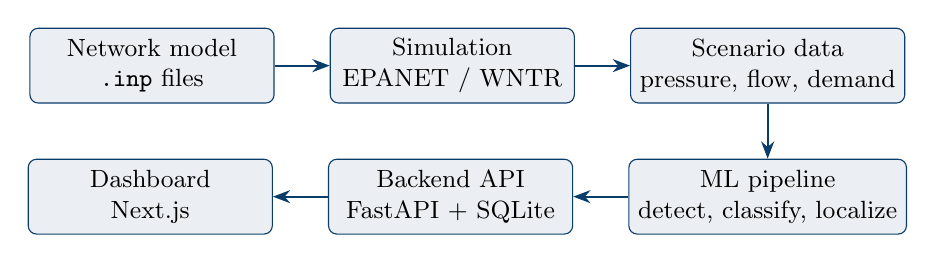
\begin{tikzpicture}[node distance=7mm,
 box/.style={draw=navy,fill=navy!8,rounded corners=3pt,minimum width=3.1cm,minimum height=0.95cm,align=center,font=\small},
 arr/.style={-{Stealth[length=2.2mm]},thick,navy}]
\node[box] (net) {Network model\\ \code{.inp} files};
\node[box,right=of net] (sim) {Simulation\\ EPANET / WNTR};
\node[box,right=of sim] (data) {Scenario data\\ pressure, flow, demand};
\node[box,below=of data] (ml) {ML pipeline\\ detect, classify, localize};
\node[box,left=of ml] (api) {Backend API\\ FastAPI + SQLite};
\node[box,left=of api] (ui) {Dashboard\\ Next.js};
\draw[arr](net)--(sim);\draw[arr](sim)--(data);\draw[arr](data)--(ml);\draw[arr](ml)--(api);\draw[arr](api)--(ui);
\end{tikzpicture}
\caption{End-to-end pipeline: from network models to the user's screen.}\label{fig:arch}\end{figure}

The repository is organised as a monorepo (Appendix~\ref{app:tree}): \code{simulation/} builds scenarios and runs the simulator; \code{ml\_pipeline/} holds data loading, features, detector, classifier, localizer and evaluation; \code{backend/} exposes the results; \code{frontend/} is the dashboard; \code{data/} holds networks, simulated scenarios and result files.

\section{Simulation and Data}
\subsection{Networks}
\begin{center}\small\begin{tabular}{@{}lccccc@{}}\toprule
Network & Junctions & Pumps & Tanks & Reservoirs & Scenarios \\\midrule
Net1 & 9 & 1 & 1 & 1 & 145 \\
Net2 & 35 & 0 & 1 & 0 & 161 \\
Net3 & 92 & 2 & 3 & 2 & 281 \\\bottomrule\end{tabular}\end{center}
All are standard EPANET benchmark models. Net2 has a negative-demand junction that acts as its supply source.

\subsection{Physics of the events}
Every scenario is a 24-hour extended-period simulation with pressure-dependent demand. A leak at node $i$ is an orifice
\begin{equation}Q_{\ell,i}(t)=C_d\,A\,\sqrt{2\,g\,P_i(t)},\qquad C_d=0.75,\label{eq:orifice}\end{equation}
with orifice area $A$ and pressure head $P_i$. A demand change multiplies the node demand pattern by a factor: $D_i(t)=D_{\text{base},i}\,m(t)\,f$. Pump outages close a pump for a window in which it normally runs; reservoir head changes add $\Delta h$ metres; tanks start at a chosen fill level or are isolated by closing their pipe; blocked pipes are closed or given a large minor loss; ageing scales the Hazen--Williams roughness coefficient $C$ in
\begin{equation}h_f=\frac{10.67\,L\,Q^{1.852}}{C^{1.852}\,d^{4.87}}.\end{equation}

\subsection{Scenario matrix}
\code{build\_scenarios.py} reads each network's own topology and writes \code{scenarios.json}, so every node, pipe, pump, tank and reservoir id is valid for its network. Blockage candidates are tested for hydraulic convergence before inclusion. The matrix has 617 scenarios:
\begin{center}\small\begin{tabular}{@{}lrp{8.5cm}@{}}\toprule
Kind & Count & Variation \\\midrule
Leak & 299 & every junction; five sizes (0.0001--0.01 m$^2$); start at 2, 8, 12, 20 h; noisy sensors; hidden behind demand surge, hydrant, blockage or pump outage \\
Demand change & 60 & node $\times$1.5/0.5, all nodes $\times$1.3/0.7, hydrant \\
Pump / reservoir & 54 & outage 2/4/6 h, head $\pm$2, 5, 10 m \\
Tank change & 60 & fill level 10--90\%, isolation \\
Blocked pipe & 48 & closed or throttled busy pipes \\
Pipe ageing & 42 & roughness $\times$0.6--0.95 \\
Normal day & 54 & noise-free and noisy \\\bottomrule\end{tabular}\end{center}

\subsection{Recorded data and noise}
For every scenario three tables are saved with one row per hour: node pressure, pipe flow and delivered node demand (what a customer meter would read; leak flow is excluded). For ``noisy'' scenarios Gaussian measurement noise is added with a fixed random seed (pressure $\pm0.05$ or $0.2$ m; flows and demands 0.5\% or 2\%). The baseline stays clean: it stands for the hydraulic model's expectation. Pump switching makes some nodes ill-conditioned: a 1\% demand probe is run, nodes swinging more than 5 m (NET3 nodes 61 and 601) and hours where most of the network swings (NET3 hour 21) are excluded from analysis. Scenarios whose hydraulics do not converge are discarded.

\subsection{Pump speed}
Pump speed changes were planned but not simulated: WNTR's own simulator supports only speed 1.0.

\section{Methodology}
\subsection{Overview}
The ML pipeline has two stages. \emph{Stage 1 (detect):} is anything above sensor noise? \emph{Stage 2 (explain):} what kind of event is it and, for a leak, where? The functions are in \code{features.py}, \code{detector.py}, \code{classifier.py}, \code{localizer.py} and \code{pipeline.py}.

\subsection{Signals}
\textbf{Pressure residual.} $r_i(t)=P^{\text{normal}}_i(t)-P^{\text{obs}}_i(t)$. A \emph{persistent} peak requires two consecutive hours: $d_i=\max_t\min\{r_i(t),r_i(t{+}1)\}$.

\textbf{Noise calibration.} From the training normal runs of each network (about 14 of 18), $\tau_P=\max\{0.1,\,4\sigma_P\}$ (about 0.5 m in all three networks). Flow, demand and unaccounted-flow noise levels are learned the same way.

\textbf{Flow balance.} At junction $i$, with pipe flows signed $+1$ into and $-1$ out of the node,
\begin{equation}\sum_p \operatorname{sign}(p,i)\,Q_p(t)=D_i(t)+Q_{\ell,i}(t).\end{equation}
Subtracting the normal day and the change in metered demand gives the \emph{unaccounted flow}
\begin{equation}u_i(t)=\sum_p\operatorname{sign}(p,i)\,\Delta Q_p(t)-\Delta D_i(t)=Q_{\ell,i}(t),\label{eq:unaccounted}\end{equation}
which is exactly the leak flow in noise-free data. Demand changes cancel because they are metered.

\subsection{Features}
Fourteen numbers summarise a scenario, all scaled by noise thresholds or by total demand so they transfer between networks.
\begin{center}\small\begin{tabularx}{\linewidth}{@{}>{\ttfamily}p{2.9cm}Y@{}}\toprule
Feature & Meaning \\\midrule
drop\_ratio & largest persistent pressure drop / $\tau_P$ \\
frac\_hit & share of junctions with a persistent drop above $\tau_P$ \\
median\_ratio & median node drop / $\tau_P$ \\
conc\_drop & share of the total drop at the worst node \\
rise\_ratio, frac\_rise & largest persistent pressure rise / $\tau_P$; share of junctions with a rise \\
flow\_frac & share of pipes with a persistent flow change above 4 noise levels \\
source\_change & change in reservoir supply / total demand \\
tank\_change & change in net tank flow / total demand \\
pump\_drop & largest relative loss of pump flow (1 = pump off) \\
unacc\_ratio, unacc\_conc & largest $u_i$ in noise units; its share of all unaccounted flow \\
demand\_frac, demand\_total & share of nodes with changed metered demand; signed total change / demand \\\bottomrule\end{tabularx}\end{center}

\subsection{Stage 1: the quiet gate}
If $\text{drop\_ratio}<1$, $\text{rise\_ratio}<1$, $\text{unacc\_ratio}<1$, $\text{flow\_frac}<0.1$ and $\text{demand\_frac}=0$, the scenario is labelled \emph{normal} and nothing else is computed. This removes false alarms from sensor noise and also means leaks below the noise cannot be detected.

\subsection{Stage 2: cause classification}
A random forest (300 trees, balanced class weights, scikit-learn) maps the 14 numbers to one of: leak, demand change, pump/reservoir, tank, blocked pipe, ageing, normal. A depth-4 decision tree is trained alongside and its rules are saved to \code{data/results/decision\_rules.txt} so the logic can be read.

\subsection{Localization}
With $A_i=u_i^{\text{peak}}/\max_ju_j^{\text{peak}}$ and $D_i=d_i/\max_jd_j$ the score is
\begin{equation}S_i=A_i+0.3\,D_i,\label{eq:score}\end{equation}
and nodes are sorted by $S_i$. If no node has an unaccounted flow above noise, only $D_i$ is used. We also tested a graph-smoothed score $S_i'=S_i+\beta\,\overline{S}_{\mathcal N(i)}$ with $\beta=0.3$ over the neighbours $\mathcal N(i)$ in the pipe graph; on the test leaks it gave no improvement and is off by default.

\subsection{Metrics}
For leak scenario $s$ with true node $n_s$ and rank $r_s$ of that node, $\text{Top-}k=\frac1N\sum_s\mathbf 1[r_s\le k]$. Localization error is the number of pipes (and metres of pipe) on the shortest path between the first-ranked node and $n_s$. Detection is scored as precision, recall, $F_1$ and false-alarm rate on ``abnormal event vs normal''. Cause classification uses accuracy, per-class precision/recall/$F_1$ and a confusion matrix on the held-out test scenarios, plus a leave-one-network-out test (train on the training scenarios of two networks, test on the test scenarios of the third).

\section{Backend}
The backend (\code{backend/}) is a FastAPI application. At start-up it creates the SQLite database \code{sql\_app.db} and rebuilds the \code{scenarios} table from the generated manifests, so the dashboard always lists exactly the scenarios that exist on disk.

\begin{center}\small\begin{tabularx}{\linewidth}{@{}>{\ttfamily}p{5.0cm}Y@{}}\toprule
Endpoint & Purpose \\\midrule
GET /api/networks & networks with number of junctions and scenarios \\
GET /api/scenarios?network= & scenario list with structured parameters (kind, node, size, noise, hidden-by, start hour) read from SQLite \\
GET /api/network?network= & nodes (id, x, y, type, elevation) and pipes for the map \\
GET /api/analyze/\{scenario\}?use\_demand\_meters= & full analysis: cause, probabilities, features, ranked leak nodes, search region, affected nodes, per-node and per-pipe metrics, ground truth \\
GET /api/evaluation & the saved evaluation summary \\\bottomrule\end{tabularx}\end{center}

\subsection{Modules}
\begin{center}\small\begin{tabularx}{\linewidth}{@{}>{\ttfamily}p{3.4cm}Y@{}}\toprule
File & Role \\\midrule
main.py & app creation, CORS, router registration, catalogue sync \\
catalog.py & reads manifests, builds readable names and structured parameters, writes SQLite \\
models.py, database.py & SQLAlchemy models (\code{scenarios}, legacy \code{simulation\_runs}) and the SQLite engine \\
schemas.py & Pydantic response models \\
routers/network\_api.py & networks, scenarios, topology \\
routers/analysis\_api.py & runs the ML pipeline for one scenario and builds the response \\\bottomrule\end{tabularx}\end{center}
The \code{scenarios} table has the columns \code{id}, \code{network}, \code{name}, \code{scenario\_group}, \code{event\_class}, \code{truth\_nodes}, \code{params\_json} and \code{csv\_dir}. Time series stay in CSV files. Scenario ids are validated against a character whitelist before any file is read. An early bug rejected ids containing \texttt{+} or \texttt{-} (36 reservoir scenarios returned HTTP 400); the whitelist now allows them and all 617 scenarios were requested successfully.

\subsection{Analysis request}
\code{/api/analyze} loads the scenario and baseline, calls \code{pipeline.analyze} (features, gate, classifier, localizer), then adds: the search region (top node and its pipe neighbours), the affected junctions, unaccounted flow in m$^3$/s, and the ground truth with hop error. Typical time per scenario is about 22 ms after the model is loaded.

\section{Frontend}
\subsection{Stack}
Next.js 16 and React 19 (client components), Tailwind CSS 4 with CSS variables for theming, React Flow for the network map, Recharts for charts and lucide-react icons.

\subsection{Design goals}
The first prototype exposed two huge dropdowns (up to 281 scenarios) and technical vocabulary. The redesign follows these principles:
\begin{itemize}[itemsep=2pt]
\item \textbf{Guided choice instead of long lists:} three steps (network, what happened, narrow it down). Leaks are found by node number, \emph{Pick on map}, size chips and condition chips; other events by search. A counter shows how many scenarios match; \emph{Surprise me} and previous/next arrows remove the need to scroll.
\item \textbf{Honest testing built in:} every scenario carries an \emph{Unseen test} or \emph{Training} tag, the picker shows unseen scenarios by default, and a verdict for a training scenario carries a warning that a correct answer proves little. The Performance tab reports only test results and shows training accuracy beside them.
\item \textbf{One-click start:} six ready-made examples on the welcome panel.
\item \textbf{Plain language:} verdict sentence, a \emph{What to do} line, and reasons written from the measurements (``22.3 litres per second leave the pipes with no customer meter recording it''). Technical details are collapsed by default.
\item \textbf{Explained terms:} dotted-underline words show a definition on hover, focus or tap; a Guide tab holds the glossary.
\item \textbf{Themes:} light and dark, following the system setting on first visit and remembered afterwards. Colours are tokens, so charts and the map follow the theme.
\item \textbf{Accessibility and responsiveness:} visible keyboard focus, labelled controls, radio-group semantics for choices, 14--15 px base text, reduced-motion support, collapsible side panels on desktop and a stacked layout on phones.
\end{itemize}

\begin{figure}[H]\centering
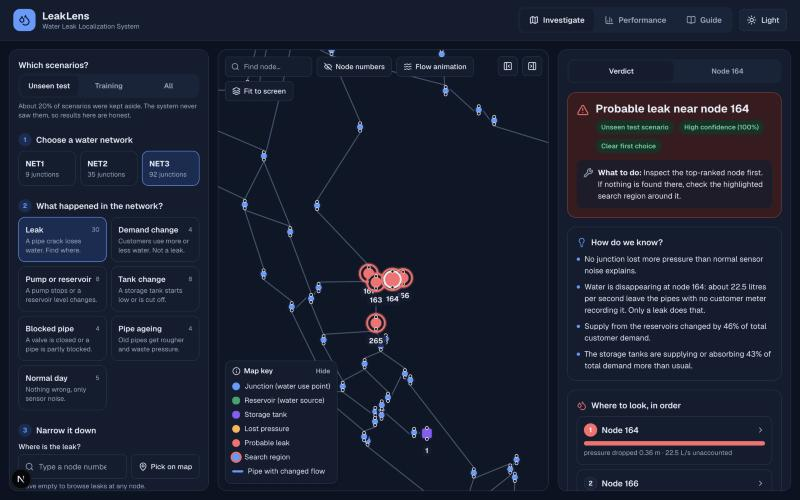
\includegraphics[width=0.98\linewidth]{figures/ui_dark_leak.jpg}
\caption{Dark theme, leak at node 115: predicted node in red with its search region, ranked list on the right.}\end{figure}
\begin{figure}[H]\centering
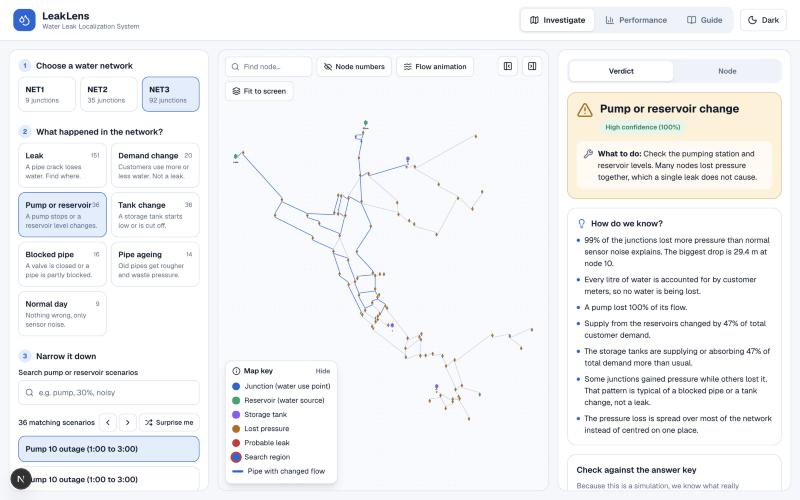
\includegraphics[width=0.98\linewidth]{figures/ui_light_pump.jpg}
\caption{Light theme, a pump outage: not a leak. Orange nodes lost pressure, blue pipes carried changed flow, and the reasons explain why the system rejects ``leak''.}\end{figure}

\subsection{Components}
\begin{center}\small\begin{tabularx}{\linewidth}{@{}>{\ttfamily}p{4.2cm}Y@{}}\toprule
Component & Role \\\midrule
app/page.tsx & layout, tabs, state, examples, analysis call \\
ScenarioPicker.tsx & three-step guided picker with filters \\
NetworkMap.tsx & map, search, key, picking mode, highlighting \\
ResultView.tsx & verdict, evidence, ranked nodes, answer key, technical details, node tab \\
PerformanceView.tsx & evaluation results in plain language \\
GuideView.tsx & how it works, glossary \\
Term.tsx, ThemeToggle.tsx & tooltips; light/dark switch \\
lib/api.ts, types.ts, glossary.ts & HTTP calls, types, definitions \\\bottomrule\end{tabularx}\end{center}

\begin{figure}[H]\centering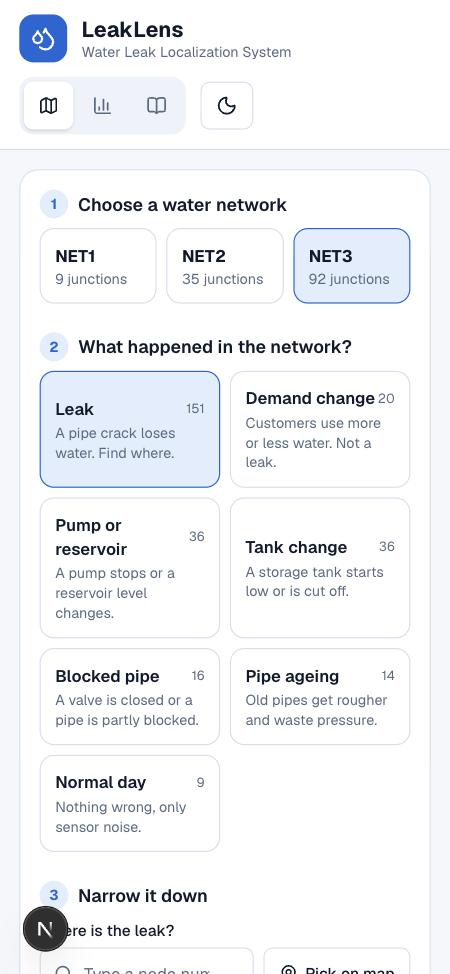
\includegraphics[width=0.46\linewidth]{figures/ui_mobile.jpg}\hspace{0.04\linewidth}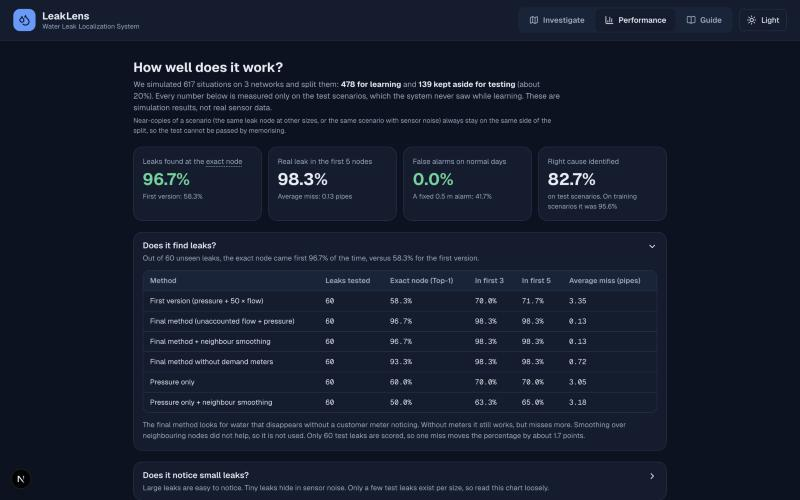
\includegraphics[width=0.46\linewidth]{figures/ui_performance.jpg}
\caption{Left: phone layout. Right: the Performance tab.}\end{figure}

\section{Evaluation and Results}
\subsection{Protocol: 80/20 hold-out}\label{sec:split}
All scenarios were split once, with a fixed seed, into about 80\% for learning (478 scenarios) and about 20\% for testing (139 scenarios, 12 of each non-leak kind and 67 leaks). The noise thresholds and the cause classifier are fitted on the training scenarios only; \textbf{every result below is measured on the test scenarios}, which the system never saw while learning. Scenarios that are near-copies stay on the same side: all leaks at one junction (every size, start time, noise level and ``hidden behind'' variant), and a scenario with its sensor-noise twin. Each network and each kind of event is split about 80/20 (code: \code{ml\_pipeline/split.py}). The dashboard tags every scenario as \emph{Unseen test} or \emph{Training}. The leak-ranking settings (weight 0.3, no smoothing) were chosen during development while looking at all scenarios, before the split existed, and were not re-tuned. The full set has 617 scenarios: 299 leak, 60 demand, 54 pump/reservoir, 60 tank, 48 blocked pipe, 42 ageing, 54 normal. Cause predictions come from the model fitted on the training scenarios. Localization uses the deterministic ranking and is scored on the 60 test leak scenarios whose node is not on the ignored list. With so few test leaks one miss moves a percentage by about 1.7 points. The first version means the Semester 1 prototype: a fixed 0.5 m detector and a score of pressure drop plus 50 times flow divergence.

\subsection{Detection}
\begin{center}\small\begin{tabular}{@{}lcccc@{}}\toprule
Method & Precision & Recall & $F_1$ & False alarms \\\midrule
Fixed 0.5 m threshold & 95.7\% & 87.4\% & 91.4\% & 41.7\% \\
Adaptive pressure detector & 100.0\% & 77.2\% & 87.1\% & 0.0\% \\
Detector + cause classifier & 100.0\% & 93.7\% & 96.7\% & 0.0\% \\
\bottomrule\end{tabular}\end{center}
The fixed threshold raised an alarm on 41.7\% of normal days because it ignores sensor noise; the learned threshold and gate raise none.

\subsection{Localization}
\begin{center}\small\begin{tabular}{@{}lcccccrr@{}}\toprule
Method & $n$ & Top-1 & Top-3 & Top-5 & Hops & $\le$1 hop & Metres \\\midrule
First version (pressure + 50 $\times$ divergence) & 60 & 58.3\% & 70.0\% & 71.7\% & 3.35 & 58.3\% & 1774 \\
Final method & 60 & 96.7\% & 98.3\% & 98.3\% & 0.13 & 96.7\% & 60 \\
Final + graph smoothing & 60 & 96.7\% & 98.3\% & 98.3\% & 0.13 & 96.7\% & 60 \\
Final, no demand meters & 60 & 93.3\% & 98.3\% & 98.3\% & 0.72 & 93.3\% & 303 \\
Pressure only & 60 & 60.0\% & 70.0\% & 70.0\% & 3.05 & 61.7\% & 1208 \\
Pressure only + smoothing & 60 & 50.0\% & 63.3\% & 65.0\% & 3.18 & 58.3\% & 1244 \\
\bottomrule\end{tabular}\end{center}
\begin{figure}[H]\centering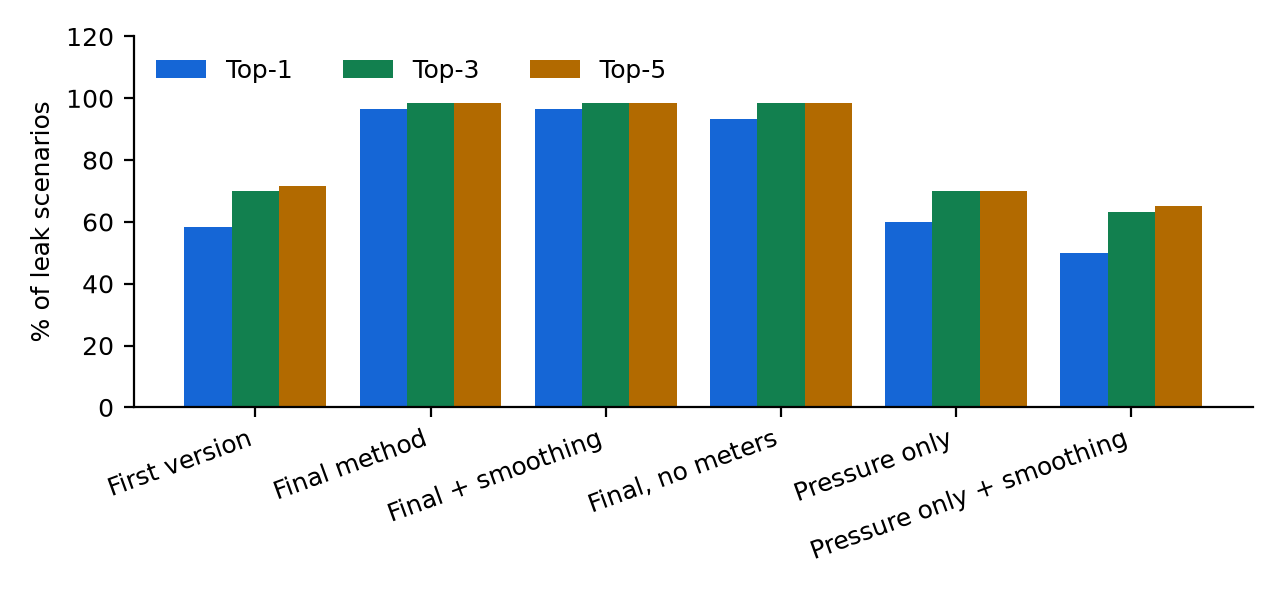
\includegraphics[width=0.85\linewidth]{figures/fig_localization.png}\caption{Localization accuracy by method.}\end{figure}
Findings: (i) unaccounted flow lifts Top-1 from 58.3\% to 96.7\%; (ii) without demand meters Top-1 is lower; (iii) pressure alone is much weaker; (iv) smoothing over graph neighbours gave no improvement (96.7\%), so network distance is used for the error metric and the search region rather than for score smoothing. End-to-end (classified as a leak and Top-1 correct): 96.7\%.

\begin{center}\small\begin{tabular}{@{}lcccc@{}}\toprule
Group & Leaks & Top-1 & Top-5 & Hops \\\midrule
Leak hidden behind another event & 10 & 100.0\% & 100.0\% & 0.00 \\
Leak with sensor noise & 4 & 100.0\% & 100.0\% & 0.00 \\
Leak size sweep & 20 & 90.0\% & 95.0\% & 0.40 \\
Leak start time & 4 & 100.0\% & 100.0\% & 0.00 \\
Leak at every junction & 22 & 100.0\% & 100.0\% & 0.00 \\
\midrule
dead-end & 17 & 100.0\% & 100.0\% & 0.00 \\
hub & 1 & 100.0\% & 100.0\% & 0.00 \\
inline & 42 & 95.2\% & 97.6\% & 0.19 \\
net1 & 11 & 100.0\% & 100.0\% & 0.00 \\
net2 & 26 & 92.3\% & 96.2\% & 0.31 \\
net3 & 23 & 100.0\% & 100.0\% & 0.00 \\
\bottomrule\end{tabular}\end{center}

\subsection{Leak size}
\begin{center}\small\begin{tabular}{@{}cccccc@{}}\toprule
Area (m$^2$) & $n$ & Noticed by pressure & Called a leak & Top-1 & Top-5 \\\midrule
0.0001 & 4 & 75.0\% & 100.0\% & 100.0\% & 100.0\% \\
0.0003 & 4 & 100.0\% & 100.0\% & 100.0\% & 100.0\% \\
0.001 & 4 & 100.0\% & 100.0\% & 100.0\% & 100.0\% \\
0.003 & 4 & 100.0\% & 100.0\% & 100.0\% & 100.0\% \\
0.01 & 4 & 100.0\% & 100.0\% & 50.0\% & 75.0\% \\
\bottomrule\end{tabular}\end{center}
\begin{figure}[H]\centering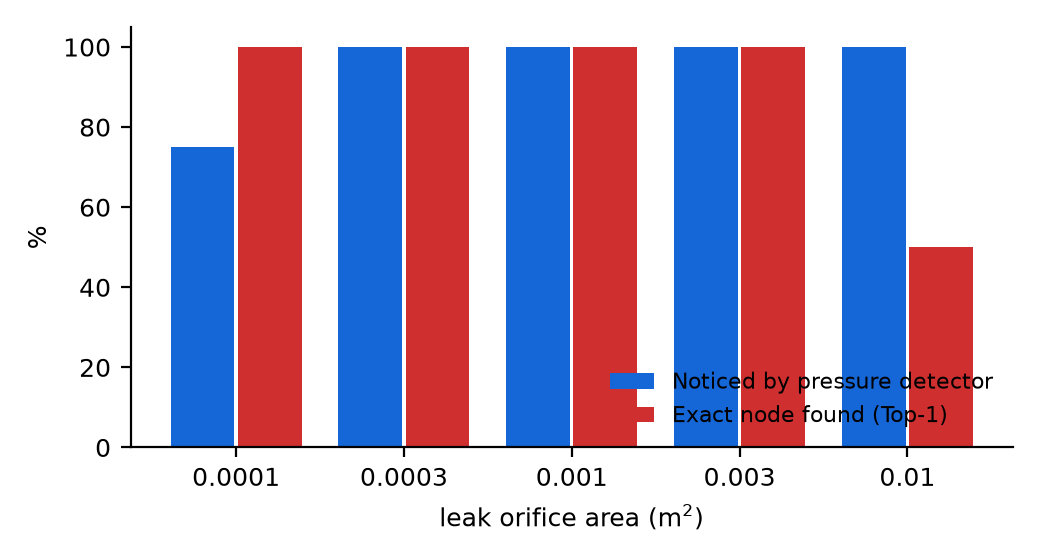
\includegraphics[width=0.6\linewidth]{figures/fig_size.png}\caption{Detection and exact-node success by leak size.}\end{figure}
Detection improves with size: 75.0\% of the smallest test leaks are noticed by the pressure detector, rising to 100\% for the larger ones. Localization is scored on every test leak whether or not detection fired. There are only four test leaks per size, so this table is indicative only. The largest leak (0.01 m$^2$) collapses pressure across the network, which makes the exact node harder to pick: 50.0\% Top-1.

\subsection{Cause classification}
Test accuracy 82.7\% (training accuracy 95.6\%), macro-$F_1$ 76.4\%, on 139 test scenarios.
\begin{center}\small\begin{tabular}{@{}lcccc@{}}\toprule
Class & Precision & Recall & $F_1$ & Scenarios \\\midrule
Normal & 60.0\% & 100.0\% & 75.0\% & 12 \\
Leak & 98.4\% & 89.6\% & 93.8\% & 67 \\
Demand change & 100.0\% & 100.0\% & 100.0\% & 12 \\
Pump / reservoir & 66.7\% & 66.7\% & 66.7\% & 12 \\
Tank change & 57.1\% & 66.7\% & 61.5\% & 12 \\
Blocked pipe & 100.0\% & 75.0\% & 85.7\% & 12 \\
Pipe ageing & 54.5\% & 50.0\% & 52.2\% & 12 \\
\bottomrule\end{tabular}\end{center}
\begin{figure}[H]\centering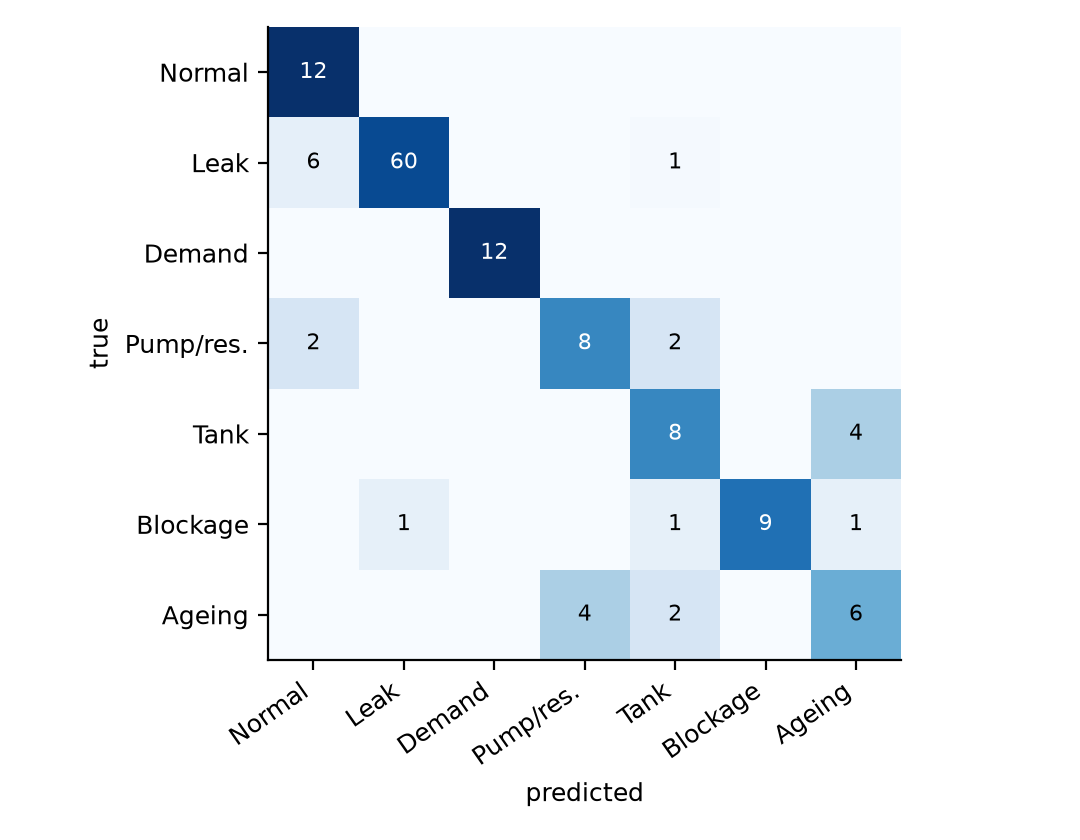
\includegraphics[width=0.58\linewidth]{figures/fig_confusion.png}\caption{Confusion matrix (counts).}\end{figure}

\subsection{Unseen networks}
\begin{center}\small\begin{tabular}{@{}lcccc@{}}\toprule
Held-out network & Accuracy & Leak recall & Leak precision & Accuracy without meters \\\midrule
NET1 & 48.5\% & 100.0\% & 100.0\% & 45.5\% \\
NET2 & 81.8\% & 92.3\% & 100.0\% & 75.0\% \\
NET3 & 54.8\% & 73.3\% & 100.0\% & 14.5\% \\
\bottomrule\end{tabular}\end{center}
Leaks transfer when demands are metered. Fine-grained non-leak causes do not yet transfer: on an unseen network pump, tank, blockage and ageing events are often confused. Without demand meters the Net3 accuracy collapses (14.5\%), because demand changes are no longer cancelled.

\section{Discussion}\label{sec:limits}
\subsection{What the results mean}
The flow-balance idea does most of the work: if each node's customer use is known, water that disappears without a meter behind it is a leak, and a demand change cancels out. This is why leak localization is so much better than with pressure alone, and why separating demand changes from leaks needs metering. The finding that graph smoothing hurts is useful: pressure drops spread to neighbours, so smoothing blurs a signal that flow balance already pins to one node.

\subsection{Limitations}
\begin{itemize}[itemsep=2pt]
\item \textbf{Simulation only.} No real sensors, real demand noise, valve operations or model errors.
\item \textbf{Demand meters assumed.} Real systems usually meter at district level, not per node; Semester 2 should estimate demands.
\item \textbf{Small leaks are not noticed} by the pressure detector and are reported as normal if every signal is within noise.
\item \textbf{Non-leak causes do not transfer across networks} reliably; in the small Net1 several causes look alike. The hold-out accuracy for causes (82.7\%) is clearly below the training accuracy (95.6\%).
\item \textbf{Small test set.} 139 test scenarios and 60 scored test leaks give wide margins of error, and the split was made once. Setting choices made earlier (ranking weight, quiet-gate cut-offs) used all scenarios and were not re-tuned.
\item \textbf{Excluded elements:} NET3 nodes 61 and 601 and hour 21; leaks at those nodes are not scored. Pump speed changes were not simulated. Some blockage candidates did not converge and were dropped.
\item \textbf{Net2 tank isolation} removes its only water source and the model calls it a leak; this case is not representative.
\end{itemize}

\subsection{Differences from the proposal}
The proposal listed noise, missing readings, changing demand, multiple leaks and cross-network testing for Semester 2. We pulled sensor noise, changing demand, operating-condition changes and cross-network testing forward because they were needed to answer the leak-versus-normal question. Missing and sparse sensors, multiple simultaneous leaks, and ML/graph models remain.

\section{Conclusion and Future Work}
LeakLens shows that, in simulation, a flow-balance localizer can place a leak at the exact node in 96.7\% of 60 cases and within one pipe in 96.7\%, that a noise-aware detector removes false alarms on normal days, and that a classifier can tell leaks from several other hydraulic changes. The dashboard makes the result understandable to a non-specialist. For Semester 2 we propose: sparse and missing sensors with centrality-guided placement~\cite{leonzio2026centrality}; demand estimation for networks without nodal meters; multiple simultaneous leaks; cause classification that transfers across networks, including graph or algorithm-informed models~\cite{zhang2026aignn} compared against the interpretable baseline; and validation on public benchmark data such as LeakDB if available.

\begingroup\footnotesize
\begin{thebibliography}{9}
\raggedright
\bibitem{sousa2026review} A.~L. Sousa, A.~F. Brochado, E. Rocha, and A. Andrade-Campos, ``A state-of-the-art review of scientific, industrial, and commercial developments in water leakage management for water supply systems,'' \emph{Water Research}, vol.~299, 125853, 2026.
\bibitem{soldevila2021hybrid} A. Soldevila, G. Boracchi, M. Roveri, S. Tornil-Sin, and V. Puig, ``Leak detection and localization in water distribution networks by combining expert knowledge and data-driven models,'' \emph{Neural Comput.\ Appl.}, vol.~34, no.~6, pp.~4759--4779, 2022.
\bibitem{sun2020leak} C. Sun, B. Parellada, V. Puig, and G. Cembrano, ``Leak localization in water distribution networks using pressure and data-driven classifier approach,'' \emph{Water}, vol.~12, no.~1, 54, 2020.
\bibitem{leonzio2026centrality} D.~U. Leonzio, T. Cattai, P. Bestagini, S. Colonnese, and S. Tubaro, ``Centrality-guided node selection for efficient water leak detection,'' \emph{IEEE Access}, vol.~14, pp.~24432--24446, 2026.
\bibitem{zhang2026aignn} Z. Zhang and O. Fink, ``Algorithm-informed graph neural networks for leakage detection and localization in water distribution networks,'' \emph{Reliab.\ Eng.\ Syst.\ Saf.}, vol.~265, 111494, 2026.
\bibitem{fan2022acoustic} H. Fan, S. Tariq, and T. Zayed, ``Acoustic leak detection approaches for water pipelines,'' \emph{Automation in Construction}, vol.~138, 104226, 2022.
\bibitem{epanet} U.S.\ EPA, \emph{EPANET 2.2: Water Distribution System Hydraulic and Water Quality Modeling}.
\bibitem{wntr} U.S.\ EPA, \emph{WNTR: Water Network Tool for Resilience}.
\end{thebibliography}
\endgroup

\appendix
\section{Repository layout}\label{app:tree}
\begin{lstlisting}
BTP/
  simulation/   simulator.py  build_scenarios.py  generate_dataset.py  scenarios.json
  ml_pipeline/  dataset.py  features.py  detector.py  classifier.py
                localizer.py  pipeline.py  train.py  evaluate.py  models/
  backend/      main.py  catalog.py  models.py  schemas.py  database.py  routers/
  frontend/     src/app/page.tsx  src/components/*.tsx  src/lib/*.ts
  data/         networks/ (Net1-3.inp)  raw_simulations/<net>/  results/
  reports/      this report and figures
\end{lstlisting}

\section{How to run}
\begin{lstlisting}
python simulation/build_scenarios.py         # scenario matrix
python simulation/generate_dataset.py --force  # simulate (about 30 s)
python ml_pipeline/train.py                  # train the cause classifier
python ml_pipeline/evaluate.py               # evaluation -> data/results/
cd backend  && uvicorn main:app --port 8000  # API
cd frontend && npm install && npm run dev    # dashboard on port 3000
\end{lstlisting}

\section{Example API response (abridged)}
\begin{lstlisting}
GET /api/analyze/net3_leak_115
{ "network": "net3", "event_class": "leak", "event_label": "Leak",
  "probabilities": {"leak": 1.0, ...},
  "predicted_leaks": [{"node_id": "115", "confidence_score": 1.3,
                       "pressure_drop": 0.63, "flow_divergence": 0.0223}, ...],
  "candidate_region": ["107","111","113","115","117"],
  "scenario_truth": {"event_class": "leak", "leak_nodes": "115"},
  "localization_error_hops": 0 }
\end{lstlisting}
\end{document}
